

\tikzset{every picture/.style={line width=0.75pt}} %set default line width to 0.75pt        

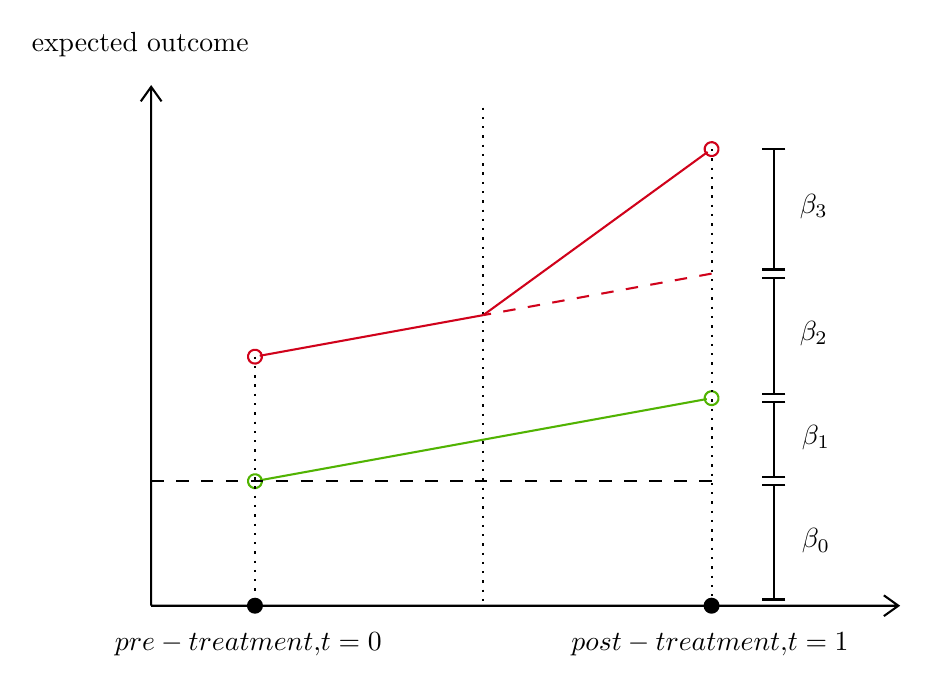
\begin{tikzpicture}[x=0.75pt,y=0.75pt,yscale=-1,xscale=1]
%uncomment if require: \path (0,466); %set diagram left start at 0, and has height of 466

%Shape: Axis 2D [id:dp8173979251061212] 
\draw  (200,320) -- (560,320)(200,70) -- (200,320) -- cycle (553,315) -- (560,320) -- (553,325) (195,77) -- (200,70) -- (205,77)  ;
%Straight Lines [id:da6661208351165583] 
\draw  [dash pattern={on 0.84pt off 2.51pt}]  (360,80) -- (360,320) ;
%Straight Lines [id:da9496708268405148] 
\draw [color={rgb, 255:red, 81; green, 179; blue, 2 }  ,draw opacity=1 ]   (252.31,259.58) -- (467.69,220.42) ;
\draw [shift={(470,220)}, rotate = 349.7] [color={rgb, 255:red, 81; green, 179; blue, 2 }  ,draw opacity=1 ][line width=0.75]      (0, 0) circle [x radius= 3.35, y radius= 3.35]   ;
\draw [shift={(250,260)}, rotate = 349.7] [color={rgb, 255:red, 81; green, 179; blue, 2 }  ,draw opacity=1 ][line width=0.75]      (0, 0) circle [x radius= 3.35, y radius= 3.35]   ;
%Straight Lines [id:da7605028786786207] 
\draw [color={rgb, 255:red, 208; green, 2; blue, 27 }  ,draw opacity=1 ]   (252.31,199.58) -- (360,180) ;
\draw [shift={(250,200)}, rotate = 349.7] [color={rgb, 255:red, 208; green, 2; blue, 27 }  ,draw opacity=1 ][line width=0.75]      (0, 0) circle [x radius= 3.35, y radius= 3.35]   ;
%Straight Lines [id:da6204156956628457] 
\draw [color={rgb, 255:red, 208; green, 2; blue, 27 }  ,draw opacity=1 ]   (468.1,101.38) -- (360,180) ;
\draw [shift={(470,100)}, rotate = 143.97] [color={rgb, 255:red, 208; green, 2; blue, 27 }  ,draw opacity=1 ][line width=0.75]      (0, 0) circle [x radius= 3.35, y radius= 3.35]   ;
%Straight Lines [id:da7633688703424713] 
\draw [color={rgb, 255:red, 208; green, 2; blue, 27 }  ,draw opacity=1 ] [dash pattern={on 4.5pt off 4.5pt}]  (470,160) -- (360,180) ;
%Straight Lines [id:da8118050967929765] 
\draw  [dash pattern={on 4.5pt off 4.5pt}]  (200,260) -- (470,260) ;
%Straight Lines [id:da5126836868598805] 
\draw    (500,262) -- (500,317) ;
\draw [shift={(500,317)}, rotate = 270] [color={rgb, 255:red, 0; green, 0; blue, 0 }  ][line width=0.75]    (0,5.59) -- (0,-5.59)   ;
\draw [shift={(500,262)}, rotate = 270] [color={rgb, 255:red, 0; green, 0; blue, 0 }  ][line width=0.75]    (0,5.59) -- (0,-5.59)   ;

%Straight Lines [id:da3500991397548453] 
\draw    (500,222) -- (500,258) ;
\draw [shift={(500,258)}, rotate = 270] [color={rgb, 255:red, 0; green, 0; blue, 0 }  ][line width=0.75]    (0,5.59) -- (0,-5.59)   ;
\draw [shift={(500,222)}, rotate = 270] [color={rgb, 255:red, 0; green, 0; blue, 0 }  ][line width=0.75]    (0,5.59) -- (0,-5.59)   ;

%Straight Lines [id:da4371401624287816] 
\draw    (500,162) -- (500,218) ;
\draw [shift={(500,218)}, rotate = 270] [color={rgb, 255:red, 0; green, 0; blue, 0 }  ][line width=0.75]    (0,5.59) -- (0,-5.59)   ;
\draw [shift={(500,162)}, rotate = 270] [color={rgb, 255:red, 0; green, 0; blue, 0 }  ][line width=0.75]    (0,5.59) -- (0,-5.59)   ;

%Straight Lines [id:da35598018492557226] 
\draw    (500,100) -- (500,158) ;
\draw [shift={(500,158)}, rotate = 270] [color={rgb, 255:red, 0; green, 0; blue, 0 }  ][line width=0.75]    (0,5.59) -- (0,-5.59)   ;
\draw [shift={(500,100)}, rotate = 270] [color={rgb, 255:red, 0; green, 0; blue, 0 }  ][line width=0.75]    (0,5.59) -- (0,-5.59)   ;

%Straight Lines [id:da32753381874785703] 
\draw  [dash pattern={on 0.84pt off 2.51pt}]  (470,100) -- (470,320) ;
\draw [shift={(470,320)}, rotate = 90] [color={rgb, 255:red, 0; green, 0; blue, 0 }  ][fill={rgb, 255:red, 0; green, 0; blue, 0 }  ][line width=0.75]      (0, 0) circle [x radius= 3.35, y radius= 3.35]   ;
%Straight Lines [id:da9408422259752088] 
\draw  [dash pattern={on 0.84pt off 2.51pt}]  (250,200) -- (250,320) ;
\draw [shift={(250,320)}, rotate = 90] [color={rgb, 255:red, 0; green, 0; blue, 0 }  ][fill={rgb, 255:red, 0; green, 0; blue, 0 }  ][line width=0.75]      (0, 0) circle [x radius= 3.35, y radius= 3.35]   ;

% Text Node
\draw (181,331.4) node [anchor=north west][inner sep=0.75pt]    {$\text{pre-treatment, } t=0$};
% Text Node
\draw (401,331.4) node [anchor=north west][inner sep=0.75pt]    {$\text{post-treatment, } t=1$};
% Text Node
\draw (511,120.4) node [anchor=north west][inner sep=0.75pt]    {$\beta _{3}$};
% Text Node
\draw (511,181.4) node [anchor=north west][inner sep=0.75pt]    {$\beta _{2}$};
% Text Node
\draw (512,231.4) node [anchor=north west][inner sep=0.75pt]    {$\beta _{1}$};
% Text Node
\draw (512,281.4) node [anchor=north west][inner sep=0.75pt]    {$\beta _{0}$};
% Text Node
\draw (141,42) node [anchor=north west][inner sep=0.75pt]   [align=left] {expected outcome};


\end{tikzpicture}